% Drawing 144/07-2 -- folder 144, batch 07, archive page 128 (PDF page 129).
% Transcription: au crayon, un réseau carré de points (une douzaine de points pleins) sur lequel sont tracées des flèches horizontales et verticales marquées $\tilde u$, $\tilde v$, et des diagonales marquées $\tilde\rho$, $\tilde\sigma$ ; en haut à droite un cadre fléché.
% Kind: square lattice of points with arrows u~, v~ and diagonals rho~, sigma~. Method 2 (schematic redraw from the facsimile). Status: partial.
% Notes: Redrawn 2026-11-12 after Michel's answer (#146): « a figure with 9 squares, then take the centers of … » (his note is cut at fifteen words). Read so: four horizontal and four vertical pencil lines cut nine squares, the nine full points are their centres, the two diagonals run from centre to centre, and the arrows lie on the inner lines. Still partial: the end of his sentence is not known. Earlier note: Re-read on a tight crop. Pencil, faint and overinked. The 3x3 grid of full points; the two diagonals through the centre computed as straight lines from corner point to corner point, the inner points of the offset grid taken on them and on the inner horizontals and verticals, so every arrow starts and ends at the same points. Horizontal arrows along the rows y of the inner points (the middle one double-headed outwards, the lowest one at the foot of the verticals), vertical arrows along the two inner columns (up from the lower inner points, down to the bottom row), the short strokes from the top-middle point and to the bottom-middle and right-middle points, the long pencil diagonal from the lower left, and the frame line with arrows at the top right. Labels \small, written along the strokes as on the page (rotated). Still differs from the facsimile: the four tilde labels are small and turned; which of u~, v~, rho~, sigma~ each is follows the earlier reading and is uncertain; which strokes carry arrowheads is a reading where the pencil is doubled. The formula Omega_{1,1} = tau^!_{1,2} above and the line below are text, not drawn. Redrawn 2026-11-09 (issue 128): to check again. Question settled by a machine pass on the facsimile, 2026-11-12 (page): two labels corrected at 600 dpi: the second label on the left vertical is sigma-tilde (beside u-tilde), and the label under the lower horizontal is rho-tilde, written upright. The faint label on the top horizontal (set rho-tilde) and a faint tilde label just right of the lower middle point remain uncertain; v-tilde is not set. Not checked by a reader.
% Coordinates: 1 unit = 1 mm = 1/100 of the crop width (bbox in page fractions: [0.08, 0.13, 0.52, 0.44]).
% Redrawn by Claude (claude-opus-5-5), issue #73, 2026-11-09; not checked by a human; not compiled (no TeX in the session).
% Rights: reproduces part of the work -- behind RENDER_TRANSCRIPTS, never published by itself.
\documentclass[tikz,border=3pt]{standalone}
\usepackage{amsmath,amssymb}
\usetikzlibrary{arrows.meta}
\tikzset{pencil/.style={black!50}, pt/.style={circle,fill,inner sep=1.4pt}, spt/.style={circle,fill,inner sep=0.8pt}}
\begin{document}
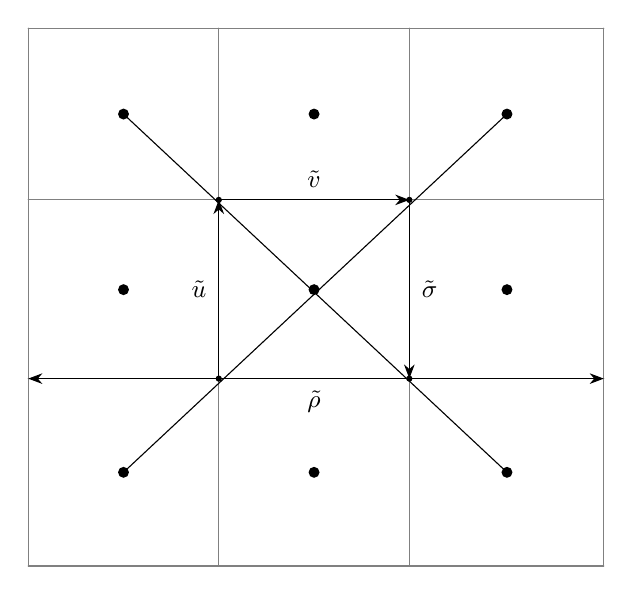
\begin{tikzpicture}[x=1mm,y=1mm,line cap=round,line join=round,font=\small,>={Stealth[length=1.8mm]}]
% The nine squares: four horizontal and four vertical lines.
\draw[pencil] (14.5,-11.6) -- (87.6,-11.6);
\draw[pencil] (14.5,-33.4) -- (87.6,-33.4);
\draw[pencil] (14.5,-56.1) -- (87.6,-56.1);
\draw[pencil] (14.5,-79.9) -- (87.6,-79.9);
\draw[pencil] (14.5,-11.6) -- (14.5,-79.9);
\draw[pencil] (38.7,-11.6) -- (38.7,-79.9);
\draw[pencil] (62.9,-11.6) -- (62.9,-79.9);
\draw[pencil] (87.6,-11.6) -- (87.6,-79.9);
% Arrows on the inner lines, as on the page.
\draw[->] (38.7,-33.4) -- (62.9,-33.4);
\draw[<->] (14.5,-56.1) -- (87.6,-56.1);
\draw[->] (38.7,-56.1) -- (38.7,-33.4);
\draw[->] (62.9,-33.4) -- (62.9,-56.1);
% The nine centres and the two diagonals through them.
\draw (26.6,-22.5) -- (75.3,-68.0);
\draw (26.6,-68.0) -- (75.3,-22.5);
\node[pt] at (26.6,-22.5) {};
\node[pt] at (26.6,-44.8) {};
\node[pt] at (26.6,-68.0) {};
\node[pt] at (50.8,-22.5) {};
\node[pt] at (50.8,-44.8) {};
\node[pt] at (50.8,-68.0) {};
\node[pt] at (75.3,-22.5) {};
\node[pt] at (75.3,-44.8) {};
\node[pt] at (75.3,-68.0) {};
% Corners of the middle square.
\node[spt] at (38.7,-33.4) {};
\node[spt] at (38.7,-56.1) {};
\node[spt] at (62.9,-33.4) {};
\node[spt] at (62.9,-56.1) {};
\node[left=1pt] at (38.7,-44.8) {$\tilde u$};
\node[above=1pt] at (50.8,-33.4) {$\tilde v$};
\node[below=1pt] at (50.8,-56.1) {$\tilde\rho$};
\node[right=1pt] at (62.9,-44.8) {$\tilde\sigma$};
\end{tikzpicture}
\end{document}
